\section{Method Claims and Evidence Levels}
\label{app:claims}
This is a research-development manuscript. The following matrix prevents the completed V7.3 system from being conflated with the new method proposal.
\begin{table*}[h]
\centering\small
\begin{tabular}{p{.23\textwidth}p{.31\textwidth}p{.37\textwidth}}
\toprule
Component & Present evidence & Missing evidence / attribution limit\\\midrule
Canonical reusable actor charts & Implemented; exported metric meshes; shared closest-point and hard-ray readout & Canonical coordinates and charts are established ideas; task formulation alone is not empirical novelty.\\
Trainable native geometry pathway & Full DPT and query training; r7 improves development hit/miss/distance against r6 & Native seeds, features and auxiliary loss change together. Free-space preservation and external confirmation remain unresolved.\\
Actual first-surface loss with constructive miss branch & Trained r6/r7; r6--r4 paired decrease in early with worse distance & A useful geometric objective, but not evidence of a new representation by itself. Silhouette and grazing behavior remain.\\
Witness-constrained chart domain & Formal representation, constraints and edge derivative in this manuscript & Boundary prediction, consistent clipped topology, observation conflicts and training are not implemented/evaluated.\\
Incidence-normalized orthogonal update & Derived; sparse gather/scatter custom adjoint; actual-mesh numerical test & Not in r7; no end-to-end optimization or learned improvement. Fixed-visibility guarantee only.\\
Sparse first-depth custom backward & Implemented BVH selection and selected-face adjoint; finite-difference and saved-tensor measurements & CPU implementation; no CUDA throughput or global visibility derivative claim.\\
\bottomrule
\end{tabular}
\caption{Method-level inventory. ``Proposed'' is a substantive specification, not an implemented result. None of these labels implies publication acceptance or overall SOTA performance.}
\end{table*}

\paragraph{What would make this a strong method claim?}
The central hypothesis is that \emph{separating support boundaries from embedding, while preserving shared first-hit witnesses, removes unsupported chart extensions without destroying useful completion}. The relevant experiment is a fixed-observation, fixed-embedding-capacity comparison of ordinary charts, orthogonal updates alone, domains alone, and their joint model. It should include literal hard queries, endpoint coverage, miss accounting, free intrusion, domain area and retained positive witnesses. Model selection remains on development data, followed by one fixed external confirmation. The current task does not launch this new training grid or modify r7.

\paragraph{Why this is more specific than another head.}
The domain changes the set of geometric points that exist, and therefore all queries of the exported surface. The witness constraint couples different observations through shared vertices; it cannot be reproduced by a scalar confidence on each ray. The sparse adjoint implements derivatives of that shared geometric query. These are the representational and mathematical commitments of the proposal. However, a learnable $b_k$ head with no support preservation and no matched evidence would still be a weak novelty claim.

\section{Derivation and Limits of the Orthogonal Constraint}
Let $e_1=v_1-v_0$, $e_2=v_2-v_0$. The selected intersection solves
\begin{equation}
 [d,-e_1,-e_2]\begin{bmatrix}t\\u\\v\end{bmatrix}=v_0-o,
 \qquad\beta=(1-u-v,u,v).
\end{equation}
Nonzero determinant is equivalent to nonzero incidence. The differential of $o+td=\sum_j\beta_jv_j$ satisfies
\begin{equation}
 d\,\delta t=\sum_j\beta_j\delta v_j+\sum_jv_j\delta\beta_j,
 \qquad\sum_j\delta\beta_j=0.
\end{equation}
The second sum lies in the original triangle's tangent plane. Multiplying by $n^\top$ gives Eq.~\ref{eq:hitjac}. No derivative of an assumed constant barycentric point was substituted for this argument. The barycentric changes disappear because the tangent-plane term is orthogonal to $n$.

For an SVD $B=U\Sigma V^\top$, $B^\dagger B$ projects onto the span of right singular vectors with nonzero singular values. Consequently
\begin{equation}
 B(I-B^\dagger B)=0,\qquad
 \langle (I-B^\dagger B)g,B^\dagger c\rangle=0.
\end{equation}
When $B$ has dependent rows, $BB^\dagger c$ is only the projection of the desired depth correction onto the feasible constraint space. The residual $c-BB^\dagger c$ quantifies conflicts. Damping a normal-equation solve makes the protection approximate and must not be described as exact orthogonality. The prototype instead applies LSMR to $B^\top$ through sparse operators, checks the \emph{true} residual, and does not use the recursively reported solver residual as proof.

The sparse representation has three vertex indices and nine float coefficients per valid witness. The forward query first selects the actual front face using geometry alone; target range never chooses that face. For misses, the custom depth function returns infinity and does not manufacture gradients. A training loss must call the existing constructive branch on misses. Rays and calibration are fixed in this implementation; their derivatives are not returned.

\paragraph{Visibility remains discrete.}
Moving a triangle across a ray can change a miss to a hit discontinuously; two triangles can exchange front order. Normalization cannot repair either event. An orthogonal step also protects no unlisted ray, and a global neural weight update can affect other actors. A future trainable version may project the decoder's output update and distill it into the network, or use Jacobian-vector products through the decoder, but these are different algorithms with different guarantees. They must not be silently identified with the vertex-space prototype.

\section{A Concrete Domain-Clipping Operator}
\label{app:clip}
The proposed boundary field $b_k$ is piecewise linear on a shared intrinsic chart grid. On an edge from $u_a$ to $u_b$ with opposite endpoint signs $s_a=b(u_a)$ and $s_b=b(u_b)$, its zero crossing is
\begin{equation}
 u_*=(1-\lambda)u_a+\lambda u_b,
 \qquad\lambda={s_a\over s_a-s_b}.
\end{equation}
Within a fixed sign pattern,
\begin{equation}
 {\partial\lambda\over\partial s_a}={-s_b\over(s_a-s_b)^2},
 \qquad {\partial\lambda\over\partial s_b}={s_a\over(s_a-s_b)^2}.
\end{equation}
Each shared edge emits one crossing vertex, reused by adjacent clipped triangles. Interpolation of the piecewise-linear embedding produces the physical crossing. A face emits a triangle or quadrilateral, with a deterministic triangulation used identically in training and evaluation. Storing each edge crossing once closes geometry bookkeeping and bounds storage by the chart grid size. There is no positive volume thickness or ray-specific mask.

This is an operator specification, not a completed clipping implementation. Opposite signs close to zero can create unstable derivatives; signs changing across an entire cell are a discrete topology event. A chart initialized with no positive domain receives no generated-surface attraction through an empty mesh. Keeping positive build witnesses and a nonempty coarse support is therefore essential. Reusing the old free objective without such constraints would recreate the established support-collapse failure V73-F02. Domain learning must also preserve the original metric and physical readout; it cannot improve the paper by merely thresholding away all difficult outputs.

\section{Complete Oracle and Pruning Definitions}
\begin{figure}[t]
\centering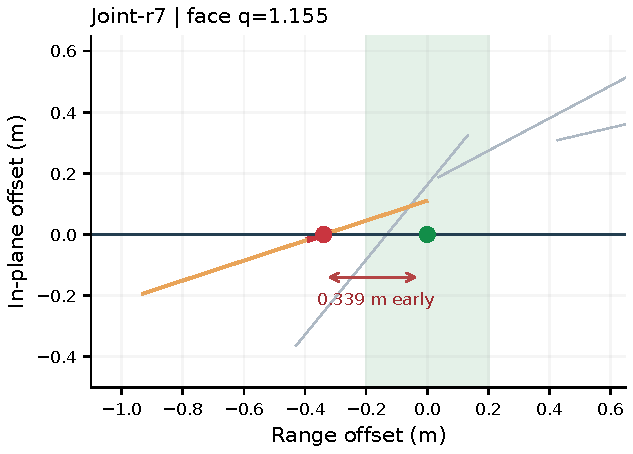
\includegraphics[width=\columnwidth]{figures/v73/r7_failure_slice.pdf}
\caption{Exact slice of the completed r7 example in Fig.~\ref{fig:blender}. The responsible regular triangle crosses 0.339\,m before the measured return. Gray shows other original triangles; the isolated chart in the Blender detail is orange here. The query uses this full surface.}
\label{fig:r7slice}
\end{figure}
The first query uses Open3D RaycastingScene's actual first intersection. All intersections and unsigned distance provide the two oracle relaxations~\cite{open3d}. These open surfaces do not justify signed-distance occupancy tests. The analysis reads original stored vertices/faces, original heldout origins/directions/ranges, and known positive-actor membership. No neural inference or optimizer update is performed. The six-method audit takes 72.70\,s on CPU. Its initial empty-frame I/O error was corrected before the complete result; no cases were discarded.

\begin{table*}[h]
\centering\small\begin{tabular}{lrrrrr}
\toprule
Method & First $\uparrow$ & Any $\uparrow$ & Near $\uparrow$ & Early $\downarrow$ & Unsupported early \\
\midrule
AdaPoinTr & 14.29 & 15.43 & 84.60 & 8.54 & 4.32 \\
VGGT native & 22.78 & 24.23 & 78.13 & 9.16 & 4.43 \\
LiDAR-R8 & 31.00 & 34.38 & 71.95 & 5.59 & 0.01 \\
Open-r3 & 31.08 & 39.04 & 69.58 & 16.22 & 1.64 \\
Attraction-r4 & 36.07 & 58.32 & 73.46 & 30.80 & 1.63 \\
First-r6 & 39.07 & 55.03 & 72.44 & 22.98 & 2.06 \\
Joint-r7 & 49.60 & 61.97 & 80.87 & 21.46 & 2.07 \\
\bottomrule
\end{tabular}

\caption{Exact oracle ladder and unsupported-component early contribution, all in percentage points of owned returns. ``Unsupported early'' is a subset of early under the stated build-component test. It is not a classifier of physical floaters.}
\end{table*}

\paragraph{Selection and rendering.}
For each method, eligible examples have at least 20 owned returns and five early returns. We select the actor whose early fraction is closest to the median among eligible actors, breaking ties by owner ID. Within that actor, an early ray with a later correct crossing is selected at median early severity when such rays exist. This intentionally visualizes a diagnosed failure class, not representative population accuracy. Raw actor counts and selection details are retained. No comparison panel is presented as a same-actor improvement unless explicitly stated.

The whole-actor Blender scene contains original surface vertices and faces. Auxiliary octahedra mark observations and cylinders mark rays; they are visualization objects only. The detail scene isolates the selected connected chart and nearby measurement markers to expose the chosen first-hit face, with no geometric smoothing, remeshing, or generated image content. Other charts are hidden only in that display. The analytic slice separately intersects every original triangle with a plane through the selected ray. This gives a checkable geometric view of the surrounding surface as well as the isolated responsibility chart.

Component support is computed as the minimum unsigned distance from any original build endpoint to that component's triangles. A 0.2\,m threshold matches the surface-recall tolerance and is not tuned per method. The shape threshold is fixed at $q>10$. Both are descriptive tests. Build-component pruning deletes all unsupported components once. The early-face oracle deletes the union of triangles selected as first early hits over owned heldout rays, then casts the same rays once against the remaining shared surface. A new front face can still be early; the oracle is not iterated to erase all violations.

\begin{figure*}[t]
\centering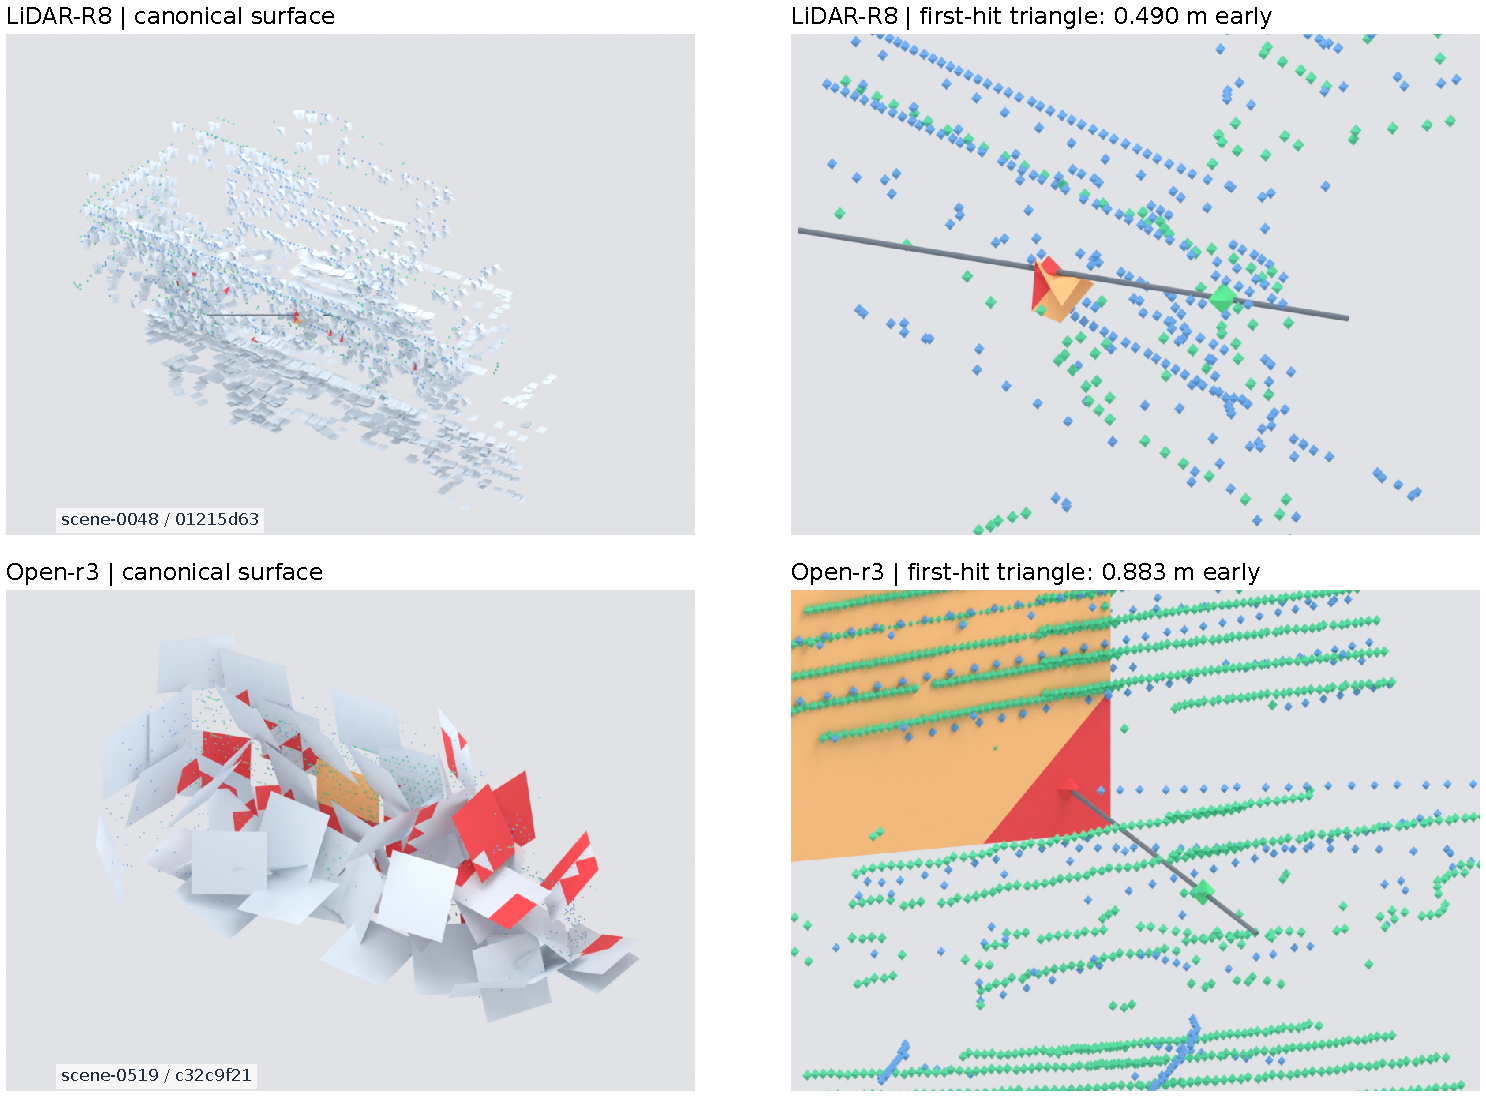
\includegraphics[width=\textwidth]{figures/v73/blender_controls_a.pdf}
\caption{Additional saved-surface renders for the LiDAR-R8 and open-chart r3 controls. The left image preserves whole-actor context and the right exposes the selected early-hit triangle. Colors and independent failure selection follow Fig.~\ref{fig:blender}. All query measurements use the full original surface.}
\end{figure*}
\begin{figure*}[t]
\centering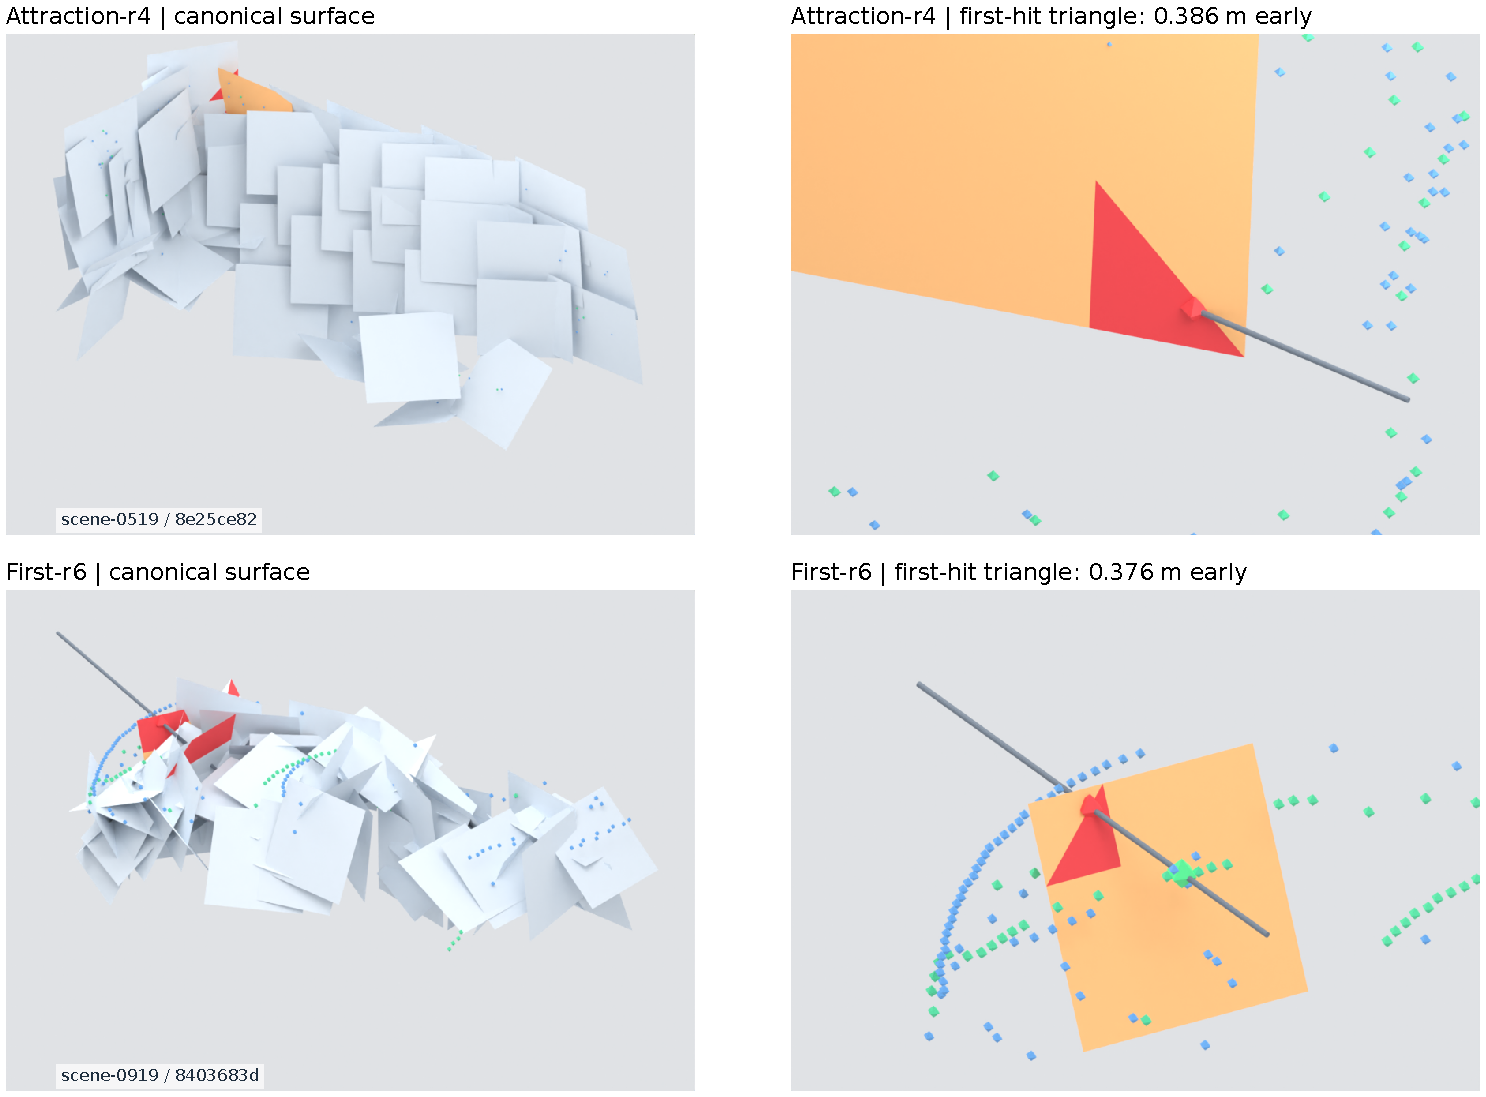
\includegraphics[width=\textwidth]{figures/v73/blender_controls_b.pdf}
\caption{Additional saved-surface renders for attraction r4 and first-surface r6. These are independently selected actors, not a matched before/after comparison. A regular chart can be locally supported while extending into the selected ray before its observed return.}
\end{figure*}

\section{Historical Results Retained as Context}
The completed V7.3 history already includes closed shared meshes, a native-only adapted DPT, short-window and full-track supervision, narrow patches, a beam free-space objective, an event objective, CAPA-style adaptation, AdaPoinTr task fine-tuning, Actor TSDF, and background composition. These comparisons establish useful failure boundaries, but combining them into one narrative does not make each an independent method contribution.

Earlier closed Q-v2 joint r1 has 7.454\,pp more early returns than its same-grid LiDAR r2, with interval $[1.122,17.719]$; the other five paired intervals cross zero. Its 67 nonempty meshes have no detected nonadjacent self-intersection, whereas the LiDAR control has such intersections in 48 of 67. Thus closed-joint failure was not directly explained by slivers or detected self-intersection. Opening the charts also did not establish joint coverage/physics dominance. These observations justify keeping topology, support direction, and visibility explanations separate.

\begin{table*}[h]
\centering\scriptsize\input{tables/v73/historical}
\caption{Previously completed V7.3 methods retained from the interim r4 archive. Different rows have different labels, adaptation and surface-conversion protocols. This table supplies history; the main paired conclusions use r6--r4 and r7--r6. The latest two methods appear in Table~\ref{tab:main}.}
\end{table*}

AdaPoinTr uses its full 32,494,657-parameter architecture, 512 queries and 16,384 output points, initialized from the official PCN checkpoint and task-fine-tuned for 30 epochs. The task interface swaps the project's Z-up coordinates to PCN Y-up and back, using known actor size for isotropic scaling. Its common-budget physical output selects centers by FPS and constructs PCA patches with fixed spacing. This conversion is part of the evaluated pipeline. A saved density diagnostic that instead uses all output points raises hit by 24.72\,pp and early by 30.85\,pp, with 0.2190\,m more free intrusion. More rendered support is not unconditionally better.

Static background composition can dominate full-scene errors and must be isolated. Existing development background TSDF/carving reduces free intrusion while increasing missing returns. The actor task does not turn an unobserved region uncovered by an edit into known background truth. Trajectory edits provide an interface demo only. External confirmation uses Argoverse~2~\cite{av2}; it is cross-dataset, not an i.i.d. nuScenes test.

\section{Reproducibility and Remaining Evaluation}
The source branch is \path{research/worldsim-v7.3-geometric-adaptation}. The completed r7 training code is 185bc728; its full DEV summary was generated once after completion and its ledger was committed as 6499d34d. Run identities are retained, without extra checksums or fingerprints. The two primary runs are:
\begin{itemize}
 \item r6: \path{WS-V73-Q-V2-01/20260909T123000Z__open-charts-lidar-first-surface-s7304-r6}.
 \item r7: \path{WS-V73-Q-V2-01/20260909T131000Z__open-charts-joint-first-surface-s7304-r7}.
\end{itemize}
All runs are beneath \path{/root/autodl-tmp/runs/worldsim_v73/}. The paired DEV evidence is \path{docs/autoresearch/worldsim_v73/ray_support/first_surface_r6_analysis.json} and \path{open_joint_r7_analysis.json} in that same evidence directory. The six-method forensics is stored under \path{docs/autoresearch/worldsim_v73/paper_forensics/20260909T184200Z__saved-surface-oracles-r1/}; the r7 extension has its own run so the original six-method audit remains identifiable.

The operator check is \path{operator_check.json} inside the first forensic directory. Scripts are \path{scripts/forensic_worldsim_v73_paper_surfaces.py}, \path{scripts/forensic_worldsim_v73_paper_r7.py}, \path{scripts/render_worldsim_v73_paper_blender.py}, and \path{scripts/worldsim_v73_witness_operator_prototype.py}. The manuscript, derived plots, selected raw cases and Blender scenes are delivered together. The official Blender color-management assets must be available when rerendering.

Twenty fixed AV2 logs contain 936 actor entries, including 878 build-ready and 58 missing-input entries. Their construction was completed before quality evaluation. The original research task launched the preregistered fixed r7/r6 confirmation after DEV completion; this manuscript does not substitute its own selection or alter that run. No completed external quality result was available at this revision's evidence cutoff. External results, full-scene composition, new support-domain training and end-to-end orthogonal updates must not be inferred from the local forensics or numerical prototype.
